\documentclass{article}
\usepackage{lmodern}
\usepackage{amsmath}
\usepackage{systeme}
\usepackage{graphicx}
\graphicspath{{images/}}
\usepackage{amssymb}
\usepackage{listings}
\usepackage{hyperref}
\usepackage[T1]{fontenc}
\usepackage{fancyhdr}
\pagestyle{fancy}
\lhead{Himaja Rachakonda, Anirudhan J. Rajagopalan}

\begin{document}

\title{Web Search Engines --- Reviews-Rehashed}
\date{March 21, 2016}
\author{Himaja Rachakonda, Anirudhan J. Rajagopalan\\ N14633788, N18824115\\ hr970, ajr619}
\maketitle
\newpage

\section{Objective}

As consumers search online for product information and to evaluate product alternatives, they often have access to dozens or hundreds of product reviews from other consumers. These customer reviews are provided in addition to product descriptions, reviews from experts, and personalized advice generated by automated recommendation systems. Each of these options has the potential to add value for a prospective customer. Online reviews have become one of the most powerful factors which impact the consumer behaviour in the E-commerce industry. Both the consumers as well as the businesses gain a ton of information from the virtual voice of reviews. Online reviews transformed the phenomenon of the simple word-of-mouth feedback into a viral form of virtual feedback, which is not only bringing immense customer satisfaction in relying on them but also showing mind boggling returns in the businesses as well. Therefore, the aim of "Reviews-Rehashed" is to make the relevant reviews more accessible to the users. 

Reviews-Rehashed is a specialized search engine to search product reviews pertaining to a product and its features. The search queries are in theform of <product,feature> tuples. This search engine will crawl reviews from various e-commerce websites such as Amazon and BestBuy.com to fetch reviews data of various products. It searches for the user query and presents the links to the results after ranking the documents based on the intrinsic quality of the document as well asthe retrieval score. The quality of the document is based on a static score derived from the features of a review like the ratings, review-date, comments etc. We have implemented the search engine for electronics - mobiles data from Amazon.com. There is a huge scope of expanding this to other products and other domains as well.

\section{Data Sources}
Amazon.com and BestBuy.com were the options considered to collect information regarding products and their reviews. To build a crawler to fetch the data, a preliminary study was conducted on the following to understand the website page layout and structure ---

\begin{enumerate}
	\item[1. ] User behaviour to search for a particular product and review.
	\item[2. ] Patterns in the URLs of the websites to reach to a particular product / product category / review / etc.
	\item[3. ] Examining the sitemap.xml of Amazon.com and BestBuy.com to get all the URLs of the domain.
\end{enumerate} 

Sitemap is a list of pages of a web site accessible to crawlers or users. It can be either a document in any form used as a planning tool for Web design, or a Web pagethat lists the pages on a Web site, typically organized in hierarchical fashion. Sitemaps make relationships between pages and other content components. It shows shapeof information space in overview. Sitemaps can demonstrate organization, navigation, and labeling system.

Sitemaps are a useful tool for making sites built in Flash and other non-html languages searchable. If a website's navigation is built with Flash, an automated search program would probably only find the initial homepage; subsequent pages are unlikely to be found without an XML sitemap.

This helped us to make sure all the review pages are searchable by our search-engine and also to find useful patterns which help in identifying each product and reviewwithin each of the domains of Amazon and BestBuy. Because of the vast expense of the data and the crawling required to be done, we have restricted our project to Amazon Review Data pertaining to Mobile Phones under Electronics Sections. This can be scaled easily to other categories and domains seamlessly with appropriate crawler jobs. 

All the review pages of a particular product with an ASIN Id can be found at a URL in the following format ---

\begin{center}
\label{sec:urlPattern}
	www.amazon.com/<Anything>/product-reviews/<ASIN>/
\end{center}

Every Review of a product has a unique Review ID, and therefore each review can be accessed by a URL in the following format ---
\begin{center}
	http://www.amazon.com/gp/customer-reviews/<Review-ID>/
\end{center}

\section{Data Collection}

Data Collection was executed in two phases ---

\begin{description}
	\item[Amazon Product Crawler: ] Fetches all the unique Ids for all mobile phone products from Amazon.com. This is required to construct the seedUrls for each product as mentioned above in the \hyperref[sec:dataSources]{Section 2},Data Sources Section.
	\item[Reviews Crawler: ] This crawler take the output of the the Amazon Product Crawler as the input to construct a seed Url for each product Id. All the unique IDs (ASINs) are stored, which are used to fetch Reviews from each product. These reviews can be accessed from this page through the links in the pagination bar. Eachpage consists of 10 reviews and the crawler goes to the depth until which there are no more review pages to be crawled for that product. Therefore, this product level URL is given as a seedURL for every product to crawl across various review pages through the links in the pagination bar.
\end{description}

The data has been collected for around 500 produts with a total of 70000 reviews. The following data about each review is collected as indexable fields based on whichthe review will be scored during the search time ---

\begin{description}
	\item[1. ] Review Content
	\item[2. ] Review Title
	\item[3. ] Review Date
	\item[4. ] Number of Comments to the review
	\item[5. ] Number of people found this review helpful
	\item[6. ] Number of images posted by the user in this review
	\item[7. ] Ratings of the review 
	\item[8. ] Is the product a Verified Purchase
	\item[9. ] Review Length
	\item[10. ] Review Id
	\item[11. ] ASIN (Product Id)
\end{description}

\section{Search Engine Architecture}
\begin{figure}[ht!]
  \centering
  \includegraphics[width=1\textwidth]{reviewsRehashedArchitecture}
  \caption{Reviews-Rehashed Search Engine Architecture\label{fig:Search_Engine}}
\end{figure}
The search engine will be built by using the following different components.
\begin{description}
  \item[Preprocessing module: ]  This module takes care of preprocessing the data and dumps the processed data into Lucene.
  \begin{description}
	 \item[Amazon WebCrawler:] This module fetches all the ASINs (unique Product Ids) for Mobile phones under Electronics Sections.
	 \item[Reviews WebCrawler:] This module fetches all the reviews of the products from the product Ids retrieved from the Amazon WebCrawler module.
  \end{description}
  \item[Document Scoring: ] This module implements the ranking algorithm by which the documents are retrieved in the search algorithm.
  \item[Retriever Service: ] This module receives the search query from the Web interface and interacts with the index store to retrieve results. The retrieved results, based on ranking algorithm in Doc Scoring module, are returned back to the web interface.
  \item[Web interface:] A web interface for the user to issue the search queries.  This will be an interface with two text boxes. One for the product name and another for the feature name.
  \item[Index store:]  This is a Lucene index store, an inverted index, which maintains all indexable data required while retrieving search results.  The data will be populated and updated periodically by a crawler job that looks for updates to the data.  The data will be stored in lucene after preprocessing.
\end{description}

\section{Document scoring}

The documents are scored based on a personalized page rank algorithm which takes the intrinsic quality of the document into consideration as well as the lucene score generated. In many search engines, we have available a measure of quality $g(d)$ for each document d that is query-independent and thus static. This quality measure may be viewed as a number between zero and one. The net score for a document d is some combination of $g(d)$ together with the query-dependent score induced by lucene. This kind of ranking algorithm demands an accumulation of an evidence of a document's relevance from multiple sources. 

The personalized pageRank algorithm gives $25\%$ weightage to the quality of the document and $75\%$ weightage to the lucene score of the document. The quality of the document is again a combination of weights given to each of the dependent facors.  

The pageRank algorithm is as follows ---

\begin{align}
pageRank(d) = 0.25 * g(d) + 0.75 * (lucene score)
\end{align}

The quality $g(d)$ of the documents is as follows 
\begin{align*}
g(d) &= 0.6 * H  + 0.20 * V + 0.13 * C + 0.07 * I, \\
 \text{where}~H: &= \text{Number of people who found the review helpful,} \\
 V: &= \text{The purchase is a verified purchase,} \\
 C: &= \text{Number of comments to the review,} \\
 I: &= \text{Number of images in the review}
\end{align*}

As all the dependent factors and the lucene score are unbounded non-negative variables with different frequency distributions, it is necessary to normalize them before we use them in the pageRank algortithm in equation (1) to have consistent scores. A sigmoid mathematical function is chosen to normalize these unbounded variables with a multiplacative factor of the x-axis to obtain scaled values between 0 and 1, based on distributions of each of these variables. 

A sigmoid function is a bounded differentiable real function that is defined for all real input values and has a positive derivative at each points range is always between 0 and 1. 
\begin{equation}
S(t) = \frac{1}{1 + e^{-t}}.
\end{equation}

The following graph shows the spread of the sigmoid function for various multpicative factors ---
\begin{figure}[ht!]
  \centering
  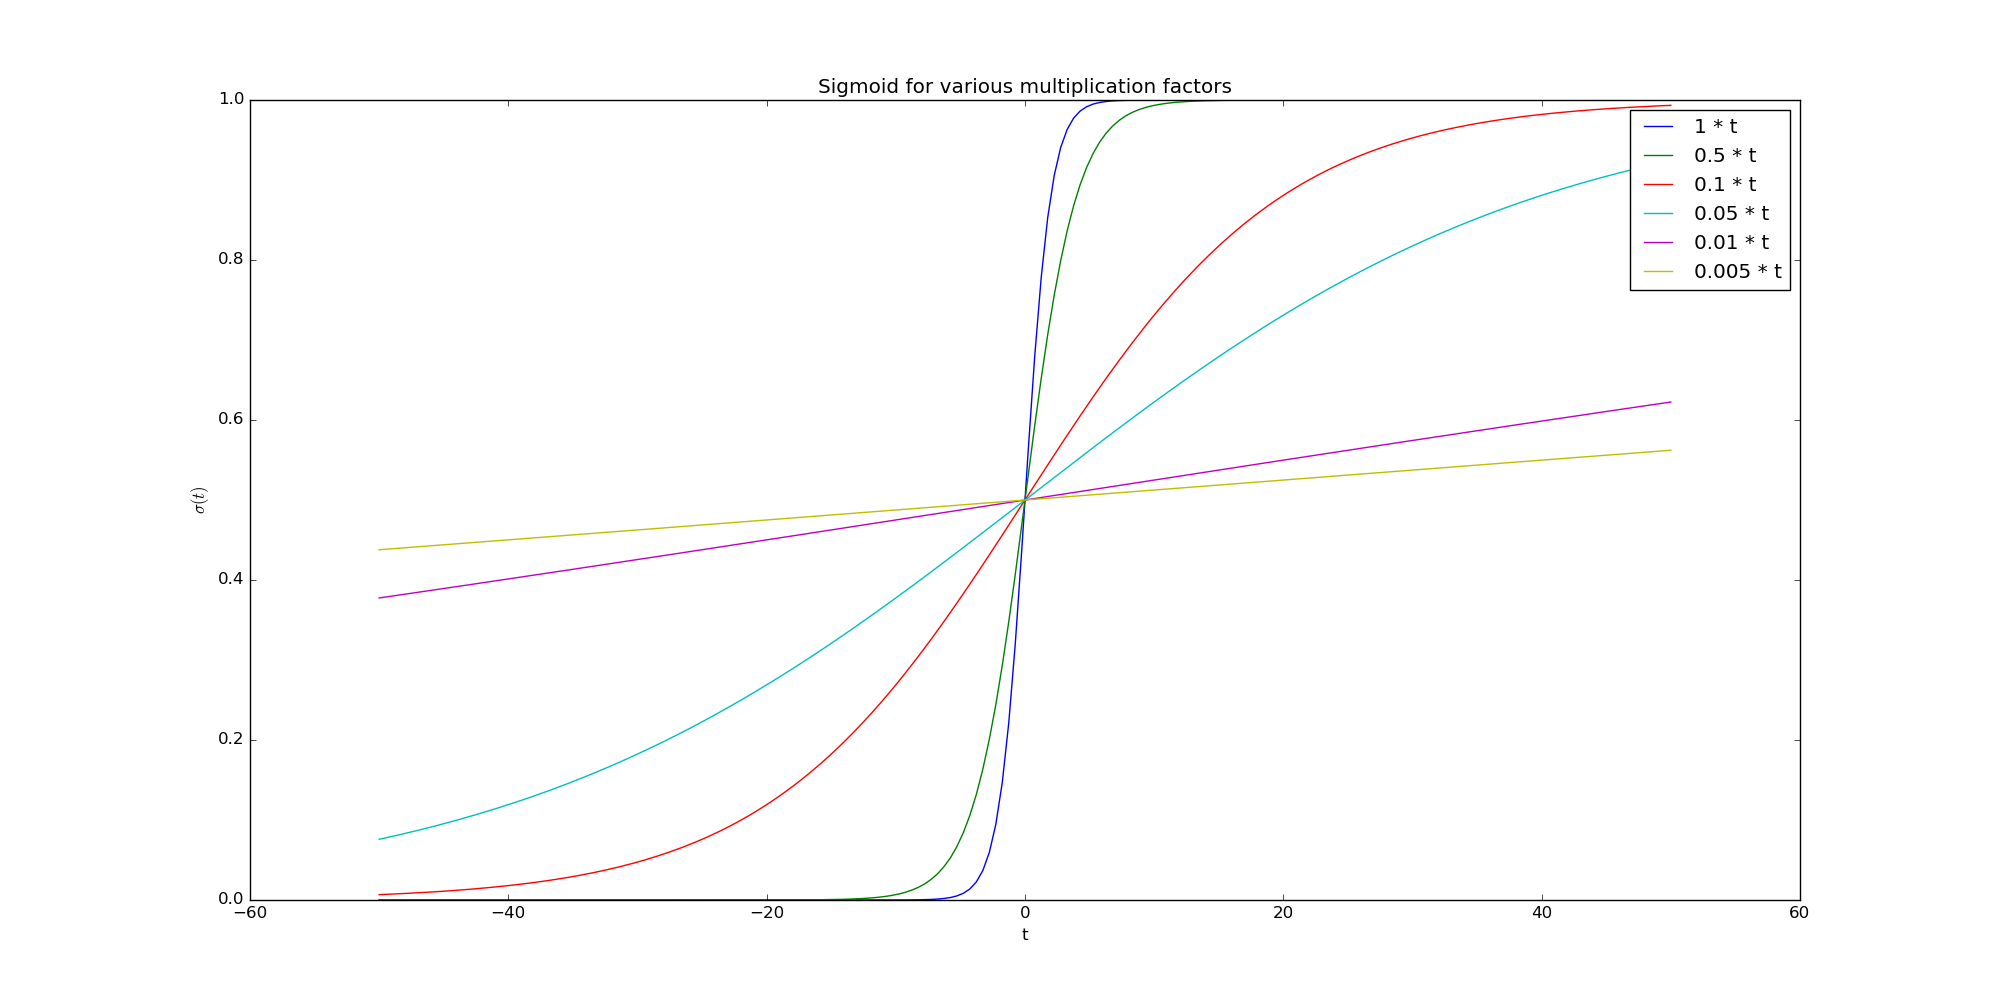
\includegraphics[width=1\textwidth]{sigmoidVariations}
  \caption{sigmoid variations with different multiplicative factors\label{fig:sigmoid}}
\end{figure}

\section{Experiments and Observations}
The reviews of the products in the search results are compared to the top reviews of those products in Amazon.com. We observed that 80\% of the times all the search results match with the top reviews of the corresponding products in Amazon. The cases where it performs well and where it doesnot perform well are discussed below--
	\begin{description}
		\item[Positive cases:] 
			\begin{description}
				\item[1 .] The best results were obtained with the final scoring formula discussed in the Section 5. This works pretty well for most of the queries with valid product name and feature name.
					\begin{figure}[ht!]
					  \centering
					  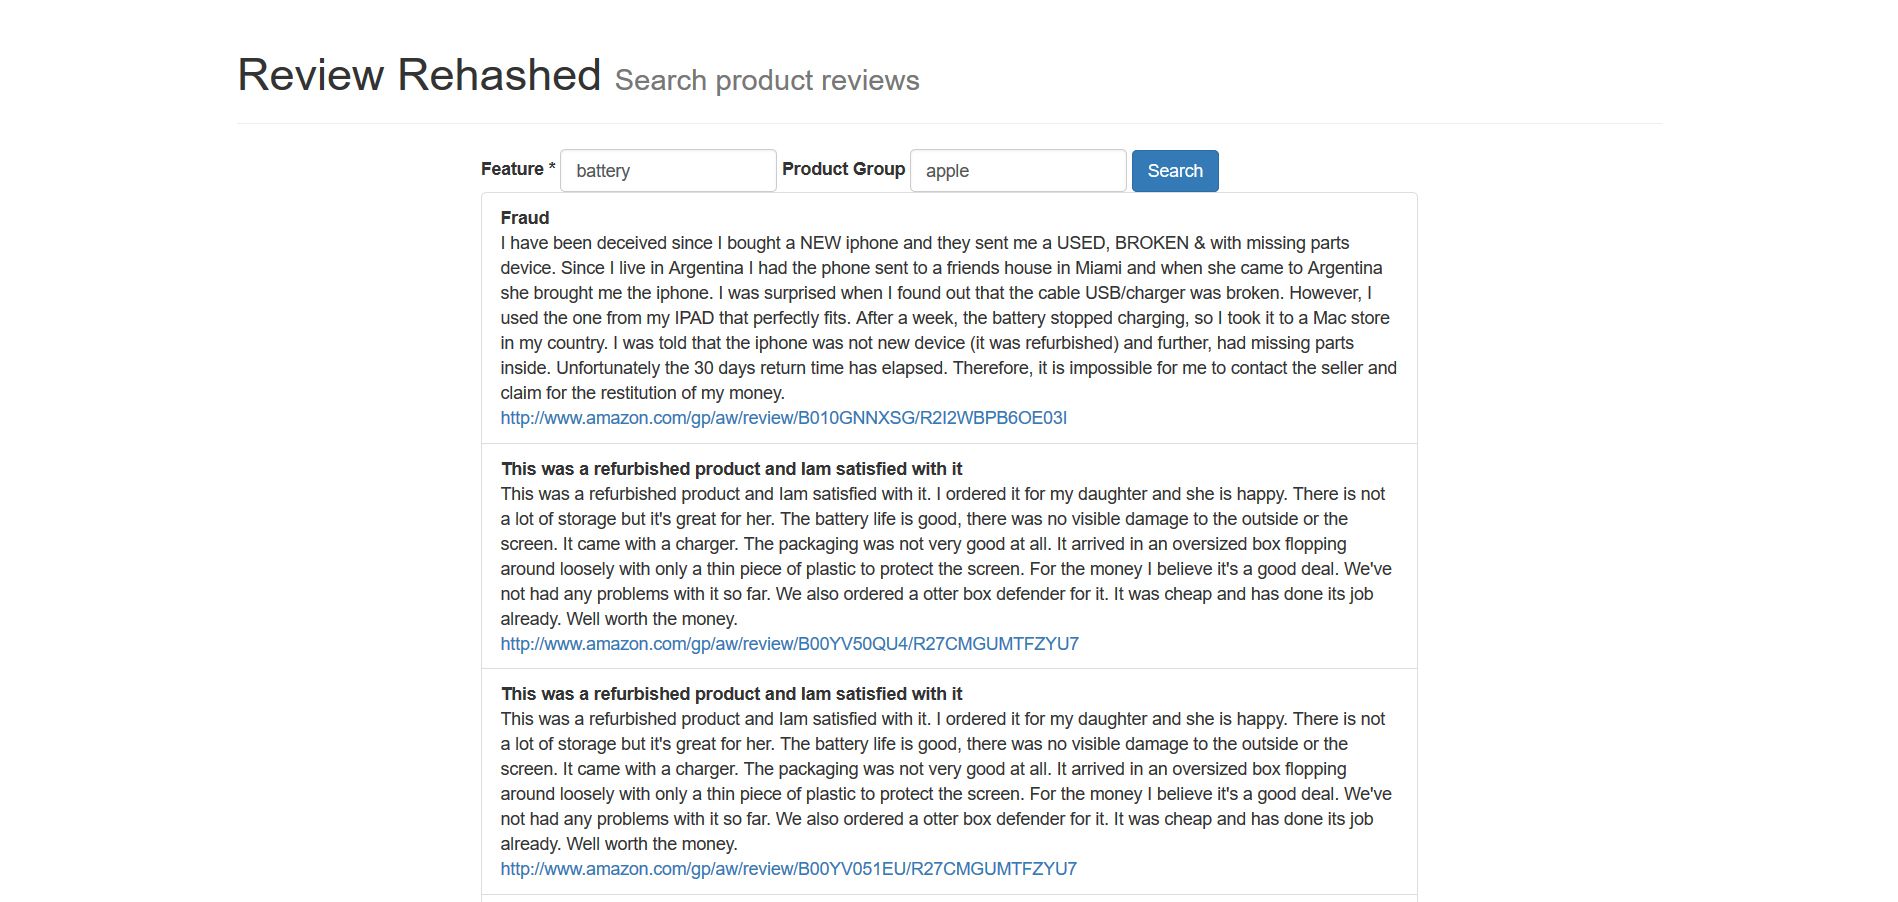
\includegraphics[width=1\textwidth]{scoring_piecewise_normalization}
					  \caption{Scoring with different multiplicative factors for the dependent factors of the score - numHelpful=0.05, isVerifiedPurchase=100, numComments=0.1, numImages=1~\label{fig:Search_Engine}}
					\end{figure}

			\end{description}
	\end{description}
%Straigh forward cases work well.
	\begin{description}
		\item[Negative cases:] 
			\begin{description}
				\item[1 .] The results are not very accurate when conjuctive queries are given in the feature, for example.
					\begin{figure}[ht!]
					  \centering
					  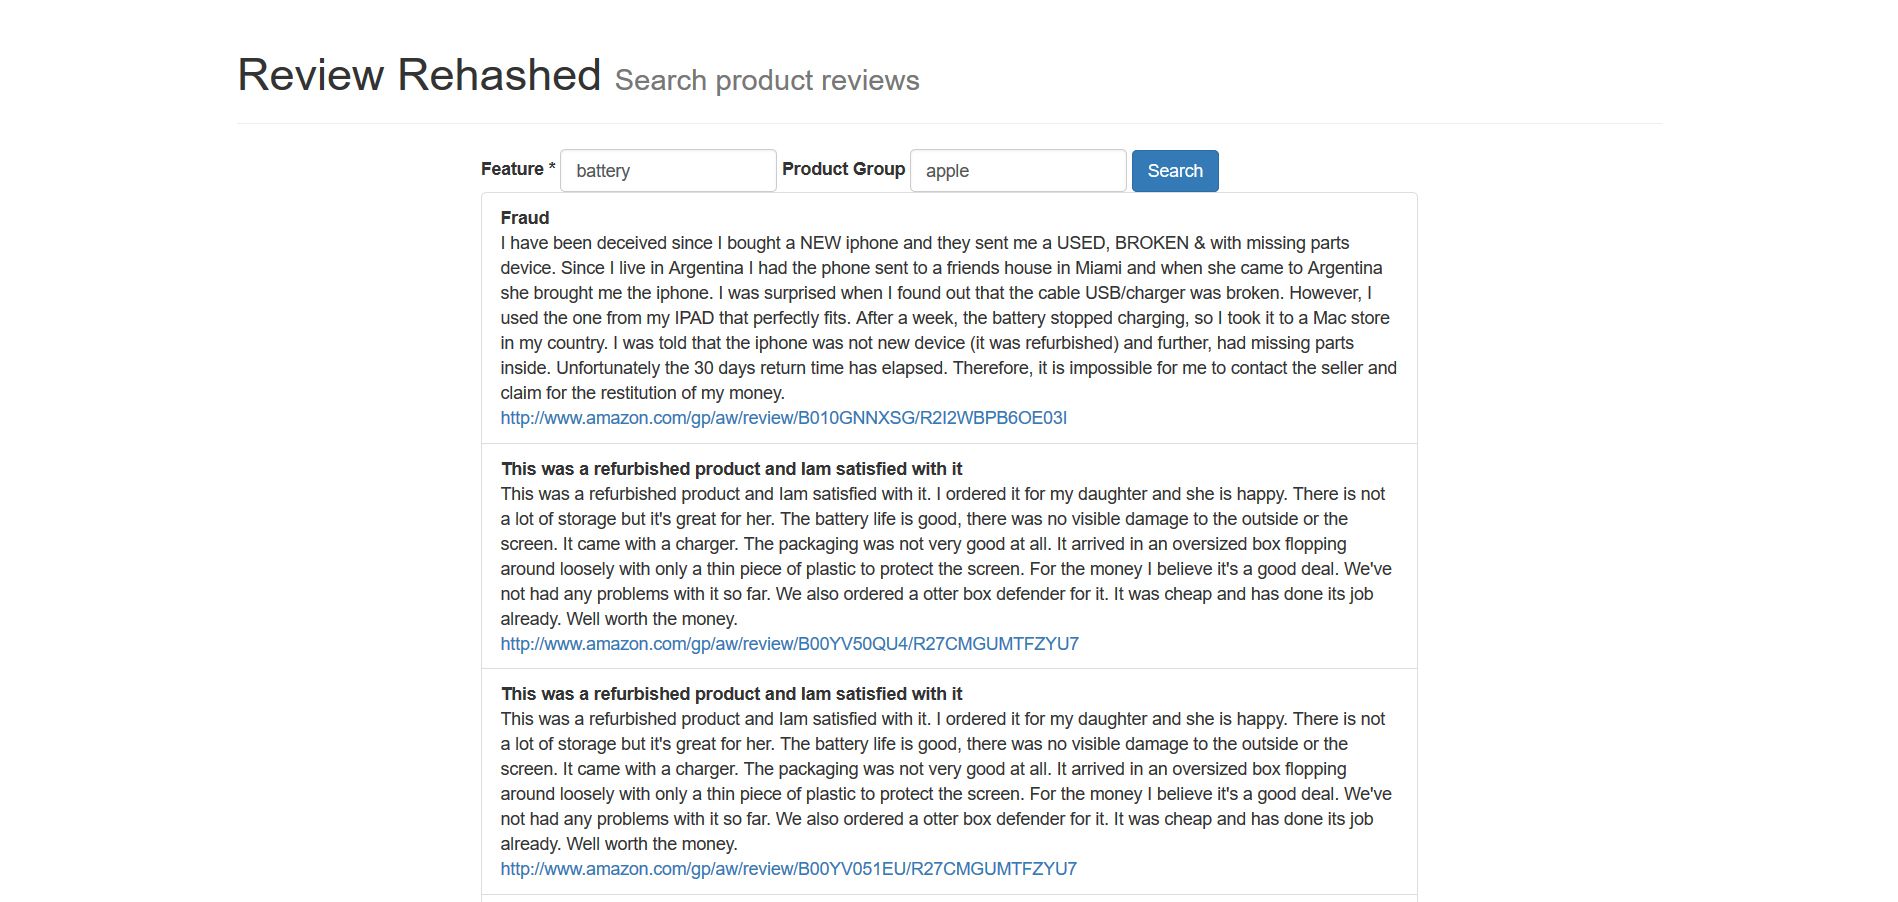
\includegraphics[width=1\textwidth]{scoring_piecewise_normalization}
					  \caption{Scoring with different multiplicative factors for the dependent factors of the score - numHelpful=0.05, isVerifiedPurchase=100, numComments=0.1, numImages=1~\label{fig:Search_Engine}}
					\end{figure}

			\end{description}
	\end{description}
cases where it does not work well
conjunctive queries within features will not show reviews with both the features discussed.
Queries with null product name do not show accurate results with current scoring mechanism, return accurate results with just lucene score. Aadjective + feature does not always return accurate results

\section{Challenges}
\begin{description}
\item Understanding patterns from sitemap.xml was a time --- taking task.
\item Manually checking the weights was a tedious task, evaluation was difficult. Have to train the data to tune these weights. (future work)
\end{description}

\section{Future work}
\begin{description}
  \item[NLP module :] This will essentially be a machine learning model that will be pre trained using the data collected by the crawler. We will use this to rank and retrieve the list of all matching sentences for a given query. This module can be developed to have the intelligence to do the following tasks--
	\begin{description}
		\item[Summary Extraction: ] A summary from the top - K reviews is presented to the user, giving an overall picture of the opinion of the crowd on this product's feature. 
		\item[Opinion Mining :] A module which shows the positive and negative reviews of a product
		\item[Data Analytics :] A module to collect data for analysis of the consumer behaviour in learning about a product and / or its features.
	\end{description}
 \item[Tuning Score parameters: ] Score Parameters can be tuned to more accurate values by training the data and running models, to improve the current scoring algorithm. Machine Learning to Rank the documents based on these parameters  may give a better performance with respect to the relevancy of the search.

\end{description}

\section{To DO}
\begin{description}
\item references
\item proof reading
\item hyper references

\begin{figure}[ht!]
  \centering
  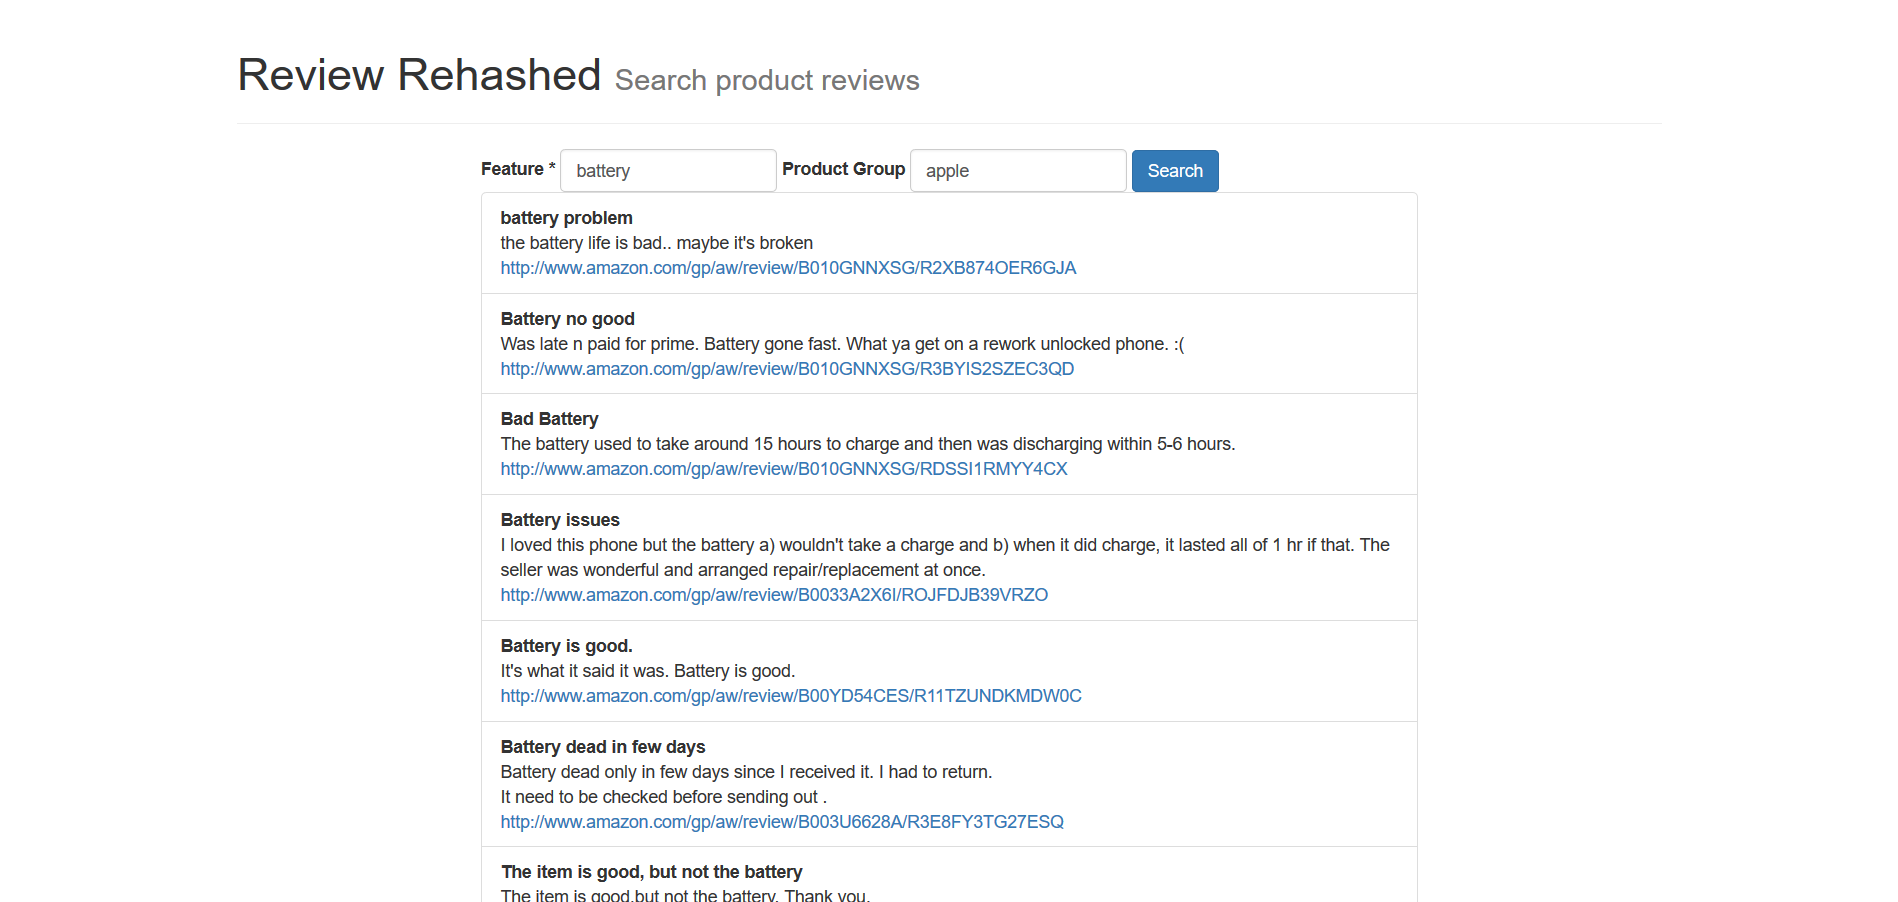
\includegraphics[width=1\textwidth]{noscoring}
  \caption{Default lucene scoring with feature query boost of 0.75 for title and 0.25 for content.~\label{fig:Search_Engine}}
\end{figure}

\begin{figure}[ht!]
  \centering
  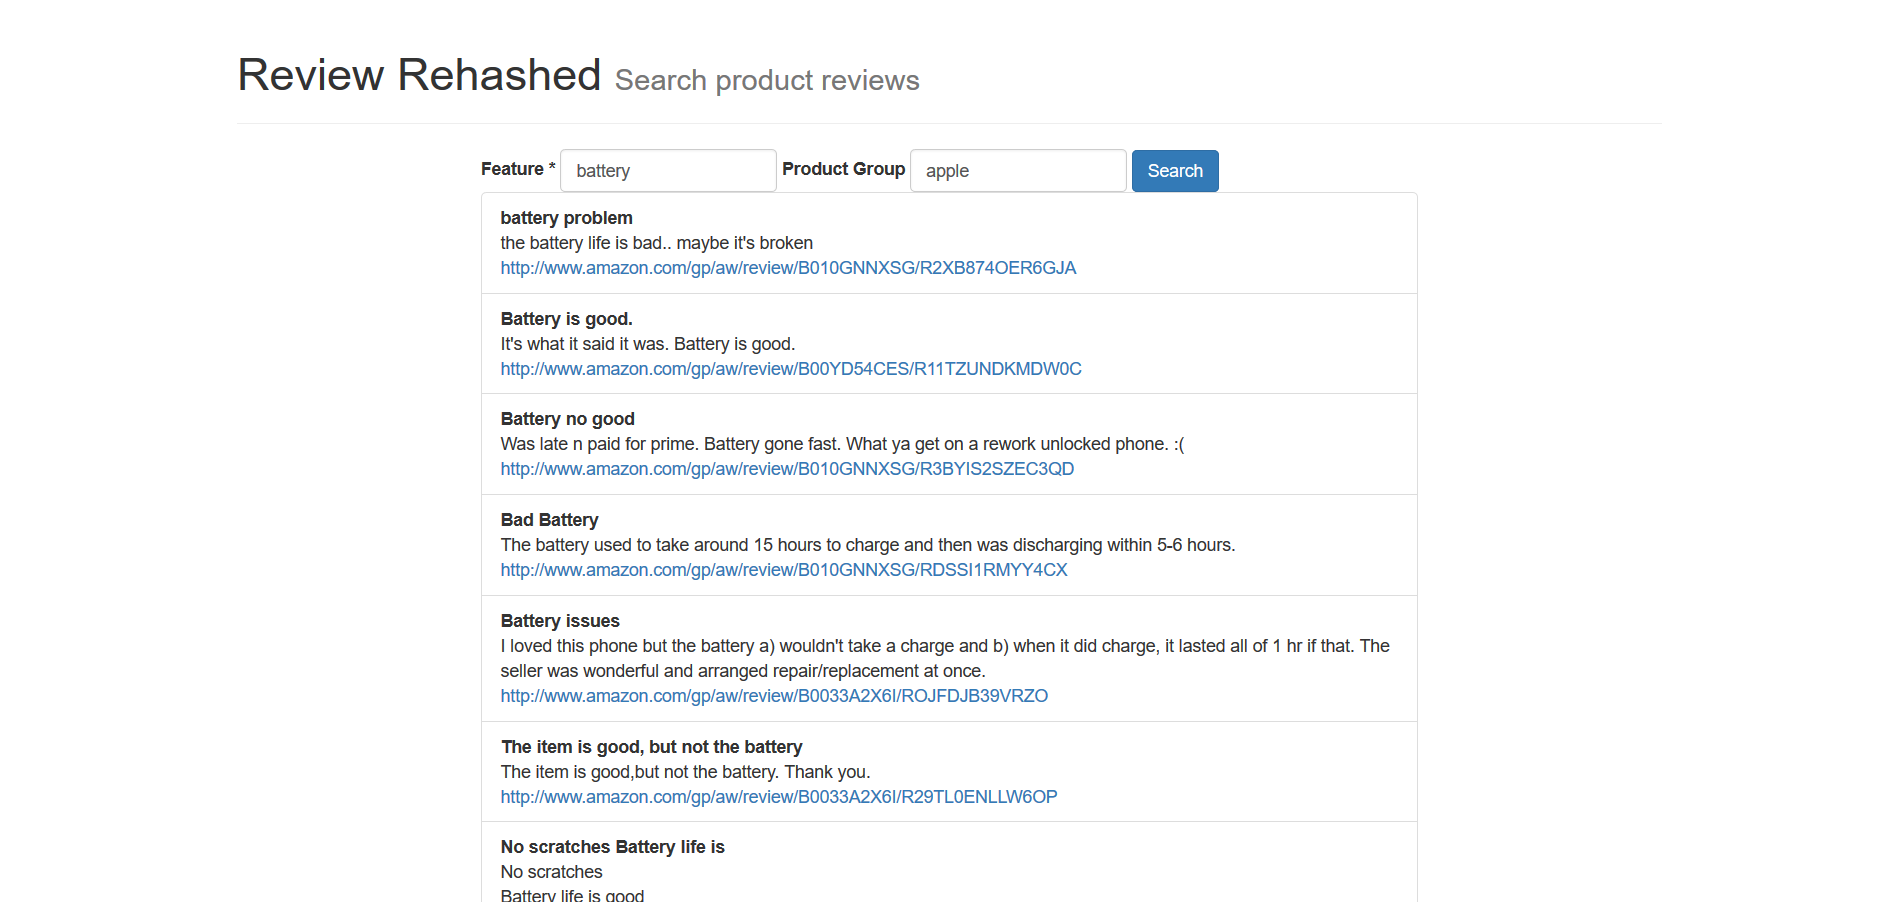
\includegraphics[width=1\textwidth]{noboosting}
  \caption{Default lucene scoring without boosting.~\label{fig:Search_Engine}}
\end{figure}

\begin{figure}[ht!]
  \centering
  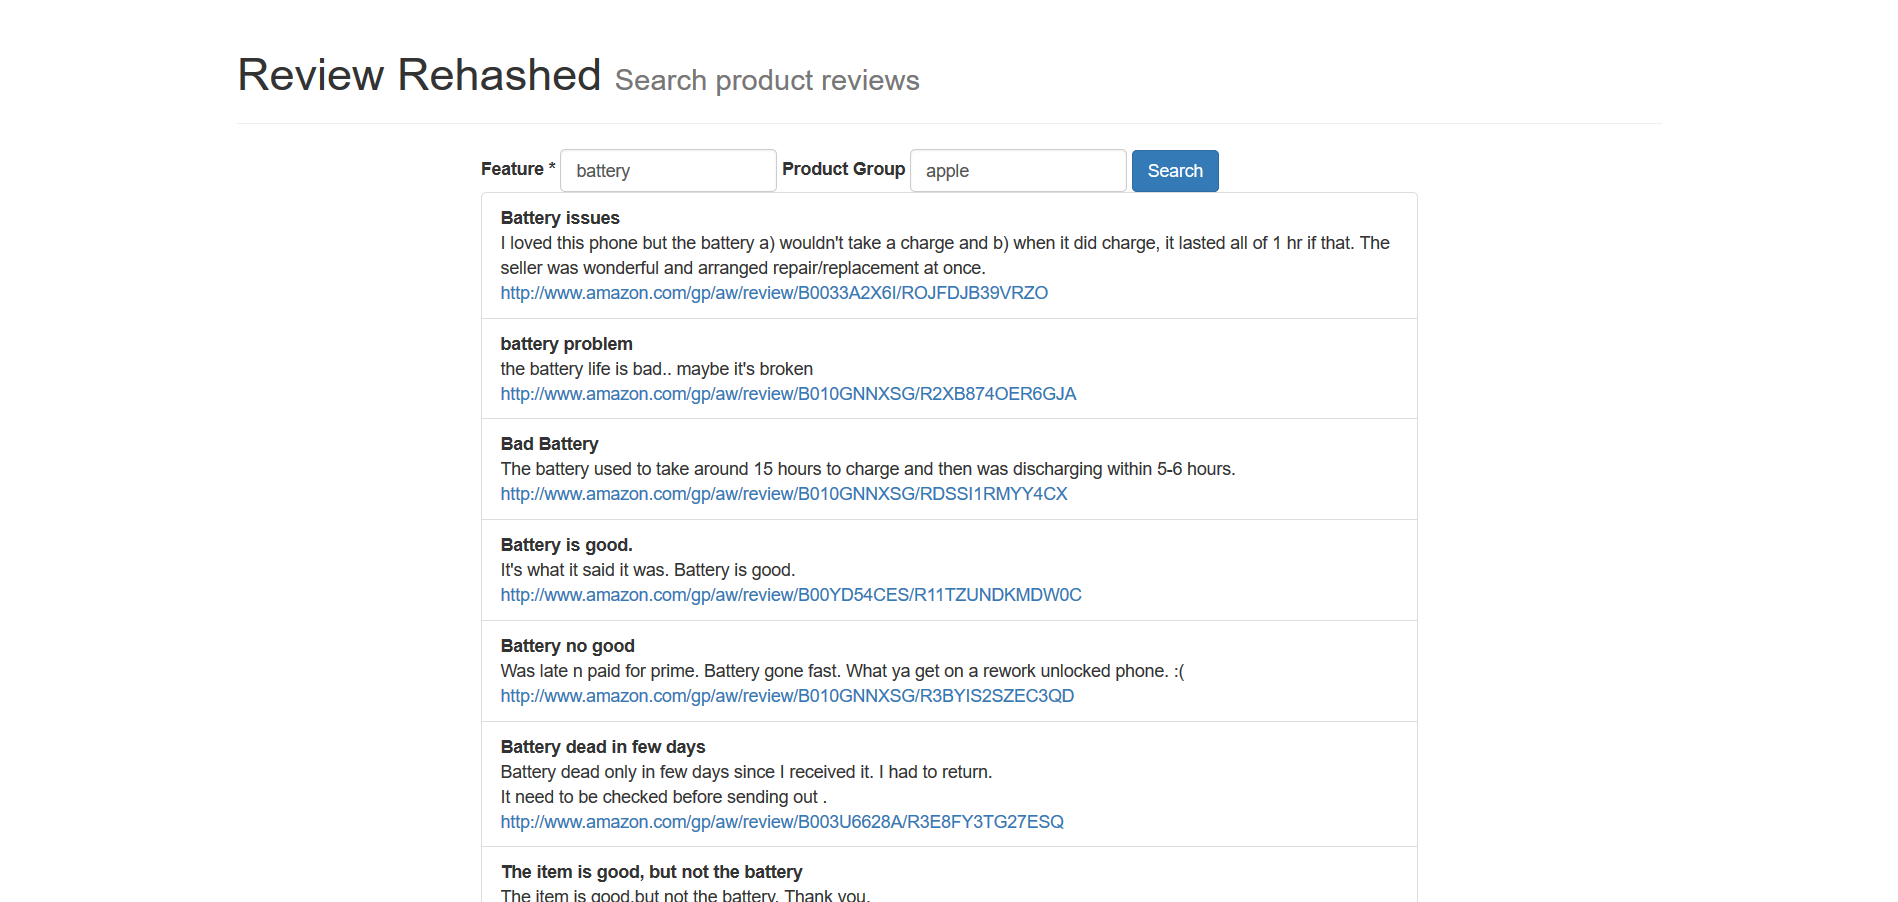
\includegraphics[width=1\textwidth]{equal_weights}
  \caption{When the normalization weights are equal.~\label{fig:Search_Engine}}
\end{figure}

\begin{figure}[ht!]
  \centering
  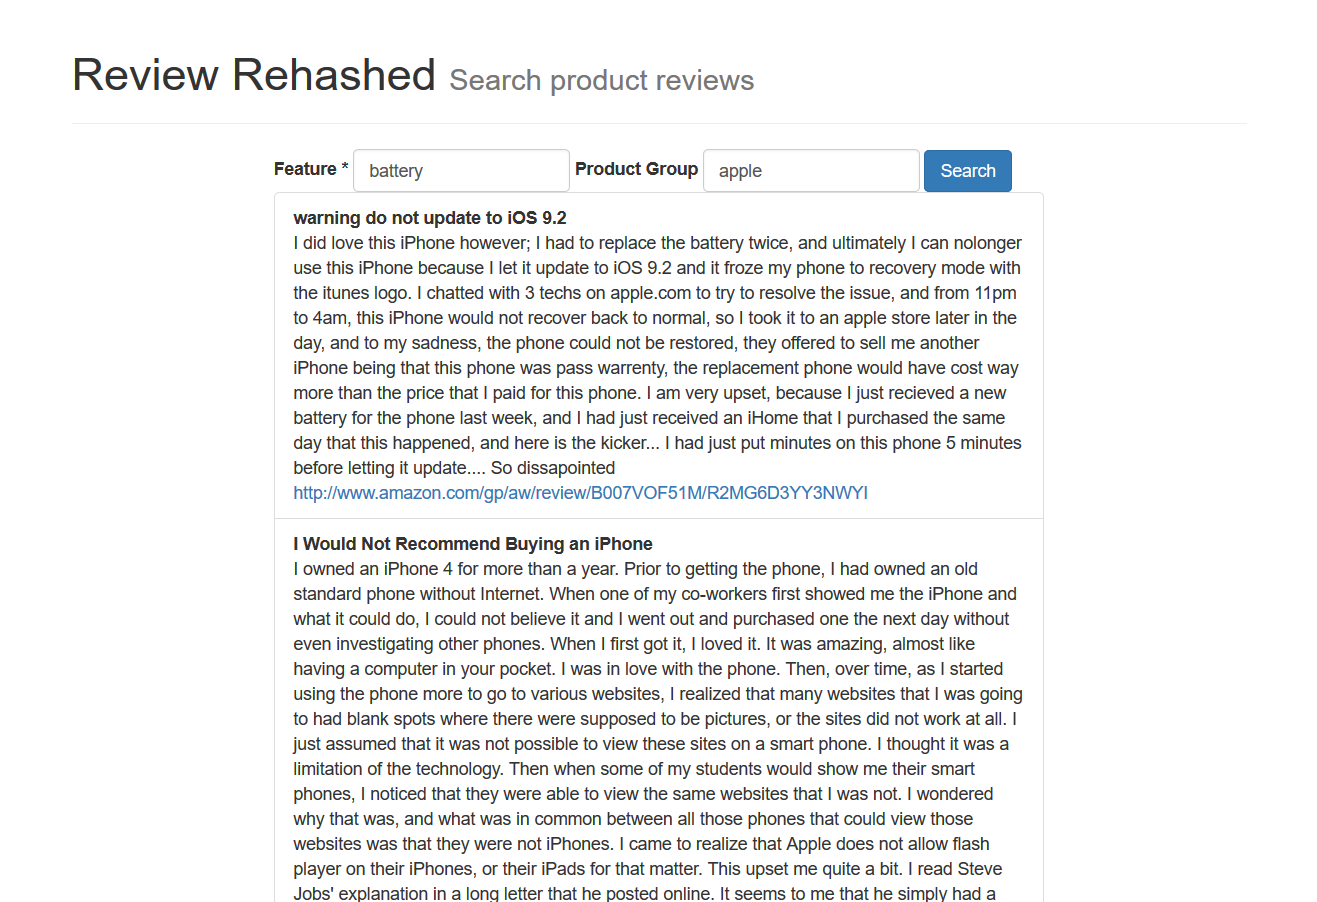
\includegraphics[width=1\textwidth]{a_new_scoring}
  \caption{This scoring is weird.  But looks decent.~\label{fig:Search_Engine}}
\end{figure}

\end{description}
\end{document}



